\documentclass[1p]{elsarticle_modified}
%\bibliographystyle{elsarticle-num}

%\usepackage[colorlinks]{hyperref}
%\usepackage{abbrmath_seonhwa} %\Abb, \Ascr, \Acal ,\Abf, \Afrak
\usepackage{amsfonts}
\usepackage{amssymb}
\usepackage{amsmath}
\usepackage{amsthm}
\usepackage{scalefnt}
\usepackage{amsbsy}
\usepackage{kotex}
\usepackage{caption}
\usepackage{subfig}
\usepackage{color}
\usepackage{graphicx}
\usepackage{xcolor} %% white, black, red, green, blue, cyan, magenta, yellow
\usepackage{float}
\usepackage{setspace}
\usepackage{hyperref}

\usepackage{tikz}
\usetikzlibrary{arrows}

\usepackage{multirow}
\usepackage{array} % fixed length table
\usepackage{hhline}

%%%%%%%%%%%%%%%%%%%%%
\makeatletter
\renewcommand*\env@matrix[1][\arraystretch]{%
	\edef\arraystretch{#1}%
	\hskip -\arraycolsep
	\let\@ifnextchar\new@ifnextchar
	\array{*\c@MaxMatrixCols c}}
\makeatother %https://tex.stackexchange.com/questions/14071/how-can-i-increase-the-line-spacing-in-a-matrix
%%%%%%%%%%%%%%%

\usepackage[normalem]{ulem}

\newcommand{\msout}[1]{\ifmmode\text{\sout{\ensuremath{#1}}}\else\sout{#1}\fi}
%SOURCE: \msout is \stkout macro in https://tex.stackexchange.com/questions/20609/strikeout-in-math-mode

\newcommand{\cancel}[1]{
	\ifmmode
	{\color{red}\msout{#1}}
	\else
	{\color{red}\sout{#1}}
	\fi
}

\newcommand{\add}[1]{
	{\color{blue}\uwave{#1}}
}

\newcommand{\replace}[2]{
	\ifmmode
	{\color{red}\msout{#1}}{\color{blue}\uwave{#2}}
	\else
	{\color{red}\sout{#1}}{\color{blue}\uwave{#2}}
	\fi
}

\newcommand{\Sol}{\mathcal{S}} %segment
\newcommand{\D}{D} %diagram
\newcommand{\A}{\mathcal{A}} %arc


%%%%%%%%%%%%%%%%%%%%%%%%%%%%%5 test

\def\sl{\operatorname{\textup{SL}}(2,\Cbb)}
\def\psl{\operatorname{\textup{PSL}}(2,\Cbb)}
\def\quan{\mkern 1mu \triangleright \mkern 1mu}

\theoremstyle{definition}
\newtheorem{thm}{Theorem}[section]
\newtheorem{prop}[thm]{Proposition}
\newtheorem{lem}[thm]{Lemma}
\newtheorem{ques}[thm]{Question}
\newtheorem{cor}[thm]{Corollary}
\newtheorem{defn}[thm]{Definition}
\newtheorem{exam}[thm]{Example}
\newtheorem{rmk}[thm]{Remark}
\newtheorem{alg}[thm]{Algorithm}

\newcommand{\I}{\sqrt{-1}}
\begin{document}

%\begin{frontmatter}
%
%\title{Boundary parabolic representations of knots up to 8 crossings}
%
%%% Group authors per affiliation:
%\author{Yunhi Cho} 
%\address{Department of Mathematics, University of Seoul, Seoul, Korea}
%\ead{yhcho@uos.ac.kr}
%
%
%\author{Seonhwa Kim} %\fnref{s_kim}}
%\address{Center for Geometry and Physics, Institute for Basic Science, Pohang, 37673, Korea}
%\ead{ryeona17@ibs.re.kr}
%
%\author{Hyuk Kim}
%\address{Department of Mathematical Sciences, Seoul National University, Seoul 08826, Korea}
%\ead{hyukkim@snu.ac.kr}
%
%\author{Seokbeom Yoon}
%\address{Department of Mathematical Sciences, Seoul National University, Seoul, 08826,  Korea}
%\ead{sbyoon15@snu.ac.kr}
%
%\begin{abstract}
%We find all boundary parabolic representation of knots up to 8 crossings.
%
%\end{abstract}
%\begin{keyword}
%    \MSC[2010] 57M25 
%\end{keyword}
%
%\end{frontmatter}

%\linenumbers
%\tableofcontents
%
\newcommand\colored[1]{\textcolor{white}{\rule[-0.35ex]{0.8em}{1.4ex}}\kern-0.8em\color{red} #1}%
%\newcommand\colored[1]{\textcolor{white}{ #1}\kern-2.17ex	\textcolor{white}{ #1}\kern-1.81ex	\textcolor{white}{ #1}\kern-2.15ex\color{red}#1	}

{\Large $\underline{12a_{0449}~(K12a_{0449})}$}

\setlength{\tabcolsep}{10pt}
\renewcommand{\arraystretch}{1.6}
\vspace{1cm}\begin{tabular}{m{100pt}>{\centering\arraybackslash}m{274pt}}
\multirow{5}{120pt}{
	\centering
	\includegraphics[width=112pt]{../../../GIT/diagram.site/Diagrams/png/1250_12a_0449.png}\\
\ \ \ A knot diagram\footnotemark}&
\allowdisplaybreaks
\textbf{Linearized knot diagam} \\
\cline{2-2}
 &
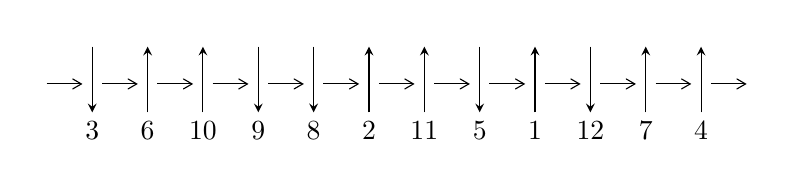
\begin{tikzpicture}[x=20pt, y=17pt]
	% nodes
	\node (C0) at (0, 0) {};
	\node (C1) at (1, 0) {};
	\node (C1U) at (1, +1) {};
	\node (C1D) at (1, -1) {3};

	\node (C2) at (2, 0) {};
	\node (C2U) at (2, +1) {};
	\node (C2D) at (2, -1) {6};

	\node (C3) at (3, 0) {};
	\node (C3U) at (3, +1) {};
	\node (C3D) at (3, -1) {10};

	\node (C4) at (4, 0) {};
	\node (C4U) at (4, +1) {};
	\node (C4D) at (4, -1) {9};

	\node (C5) at (5, 0) {};
	\node (C5U) at (5, +1) {};
	\node (C5D) at (5, -1) {8};

	\node (C6) at (6, 0) {};
	\node (C6U) at (6, +1) {};
	\node (C6D) at (6, -1) {2};

	\node (C7) at (7, 0) {};
	\node (C7U) at (7, +1) {};
	\node (C7D) at (7, -1) {11};

	\node (C8) at (8, 0) {};
	\node (C8U) at (8, +1) {};
	\node (C8D) at (8, -1) {5};

	\node (C9) at (9, 0) {};
	\node (C9U) at (9, +1) {};
	\node (C9D) at (9, -1) {1};

	\node (C10) at (10, 0) {};
	\node (C10U) at (10, +1) {};
	\node (C10D) at (10, -1) {12};

	\node (C11) at (11, 0) {};
	\node (C11U) at (11, +1) {};
	\node (C11D) at (11, -1) {7};

	\node (C12) at (12, 0) {};
	\node (C12U) at (12, +1) {};
	\node (C12D) at (12, -1) {4};
	\node (C13) at (13, 0) {};

	% arrows
	\draw[->,>={angle 60}]
	(C0) edge (C1) (C1) edge (C2) (C2) edge (C3) (C3) edge (C4) (C4) edge (C5) (C5) edge (C6) (C6) edge (C7) (C7) edge (C8) (C8) edge (C9) (C9) edge (C10) (C10) edge (C11) (C11) edge (C12) (C12) edge (C13) ;	\draw[->,>=stealth]
	(C1U) edge (C1D) (C2D) edge (C2U) (C3D) edge (C3U) (C4U) edge (C4D) (C5U) edge (C5D) (C6D) edge (C6U) (C7D) edge (C7U) (C8U) edge (C8D) (C9D) edge (C9U) (C10U) edge (C10D) (C11D) edge (C11U) (C12D) edge (C12U) ;
	\end{tikzpicture} \\
\hhline{~~} \\& 
\textbf{Solving Sequence} \\ \cline{2-2} 
 &
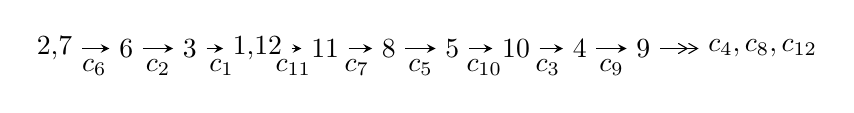
\begin{tikzpicture}[x=23pt, y=7pt]
	% node
	\node (A0) at (-1/8, 0) {2,7};
	\node (A1) at (1, 0) {6};
	\node (A2) at (2, 0) {3};
	\node (A3) at (49/16, 0) {1,12};
	\node (A4) at (33/8, 0) {11};
	\node (A5) at (41/8, 0) {8};
	\node (A6) at (49/8, 0) {5};
	\node (A7) at (57/8, 0) {10};
	\node (A8) at (65/8, 0) {4};
	\node (A9) at (73/8, 0) {9};
	\node (C1) at (1/2, -1) {$c_{6}$};
	\node (C2) at (3/2, -1) {$c_{2}$};
	\node (C3) at (5/2, -1) {$c_{1}$};
	\node (C4) at (29/8, -1) {$c_{11}$};
	\node (C5) at (37/8, -1) {$c_{7}$};
	\node (C6) at (45/8, -1) {$c_{5}$};
	\node (C7) at (53/8, -1) {$c_{10}$};
	\node (C8) at (61/8, -1) {$c_{3}$};
	\node (C9) at (69/8, -1) {$c_{9}$};
	\node (A10) at (11, 0) {$c_{4},c_{8},c_{12}$};

	% edge
	\draw[->,>=stealth]	
	(A0) edge (A1) (A1) edge (A2) (A2) edge (A3) (A3) edge (A4) (A4) edge (A5) (A5) edge (A6) (A6) edge (A7) (A7) edge (A8) (A8) edge (A9) ;
	\draw[->>,>={angle 60}]	
	(A9) edge (A10);
\end{tikzpicture} \\ 

\end{tabular} \\

\footnotetext{
The image of knot diagram is generated by the software ``\textbf{Draw programme}" developed by Andrew Bartholomew(\url{http://www.layer8.co.uk/maths/draw/index.htm\#Running-draw}), where we modified some parts for our purpose(\url{https://github.com/CATsTAILs/LinksPainter}).
}\phantom \\ \newline 
\centering \textbf{Ideals for irreducible components\footnotemark of $X_{\text{par}}$} 
 
\begin{align*}
I^u_{1}&=\langle 
b- u,\;99197 u^{26}+483399 u^{25}+\cdots+631375 a-1029892,\;u^{27}+u^{26}+\cdots+3 u+1\rangle \\
I^u_{2}&=\langle 
5.33925\times10^{205} u^{93}+1.44539\times10^{206} u^{92}+\cdots+6.46446\times10^{207} b-5.33518\times10^{207},\\
\phantom{I^u_{2}}&\phantom{= \langle  }1.10034\times10^{207} u^{93}-1.28414\times10^{208} u^{92}+\cdots+1.48683\times10^{209} a-1.01915\times10^{210},\\
\phantom{I^u_{2}}&\phantom{= \langle  }u^{94}-2 u^{93}+\cdots+239 u+23\rangle \\
I^u_{3}&=\langle 
b+u,\;3 u^{12}+2 u^{11}+10 u^{10}+5 u^9+21 u^8+9 u^7+26 u^6+8 u^5+23 u^4+2 u^3+13 u^2+a-4 u+5,\\
\phantom{I^u_{3}}&\phantom{= \langle  }u^{14}+u^{13}+4 u^{12}+3 u^{11}+9 u^{10}+6 u^9+13 u^8+7 u^7+13 u^6+5 u^5+9 u^4+u^3+4 u^2+1\rangle \\
I^u_{4}&=\langle 
- u^{13}- u^{12}-4 u^{11}-3 u^{10}-9 u^9-5 u^8-13 u^7-5 u^6-13 u^5-5 u^4-9 u^3-3 u^2+b-4 u-1,\\
\phantom{I^u_{4}}&\phantom{= \langle  }3 u^{12}+2 u^{11}+10 u^{10}+5 u^9+21 u^8+6 u^7+27 u^6+3 u^5+24 u^4+4 u^3+12 u^2+a+2 u+4,\\
\phantom{I^u_{4}}&\phantom{= \langle  }u^{14}+u^{13}+4 u^{12}+3 u^{11}+9 u^{10}+5 u^9+13 u^8+5 u^7+13 u^6+5 u^5+9 u^4+3 u^3+4 u^2+u+1\rangle \\
\\
\end{align*}
\raggedright * 4 irreducible components of $\dim_{\mathbb{C}}=0$, with total 149 representations.\\
\footnotetext{All coefficients of polynomials are rational numbers. But the coefficients are sometimes approximated in decimal forms when there is not enough margin.}
\newpage
\renewcommand{\arraystretch}{1}
\centering \section*{I. $I^u_{1}= \langle b- u,\;9.92\times10^{4} u^{26}+4.83\times10^{5} u^{25}+\cdots+6.31\times10^{5} a-1.03\times10^{6},\;u^{27}+u^{26}+\cdots+3 u+1 \rangle$}
\flushleft \textbf{(i) Arc colorings}\\
\begin{tabular}{m{7pt} m{180pt} m{7pt} m{180pt} }
\flushright $a_{2}=$&$\begin{pmatrix}0\\u\end{pmatrix}$ \\
\flushright $a_{7}=$&$\begin{pmatrix}1\\0\end{pmatrix}$ \\
\flushright $a_{6}=$&$\begin{pmatrix}1\\u^2\end{pmatrix}$ \\
\flushright $a_{3}=$&$\begin{pmatrix}u\\u^3+u\end{pmatrix}$ \\
\flushright $a_{1}=$&$\begin{pmatrix}u^3\\u^5+u^3+u\end{pmatrix}$ \\
\flushright $a_{12}=$&$\begin{pmatrix}-0.157113 u^{26}-0.765629 u^{25}+\cdots+2.13457 u+1.63119\\u\end{pmatrix}$ \\
\flushright $a_{11}=$&$\begin{pmatrix}-0.157113 u^{26}-0.765629 u^{25}+\cdots+1.13457 u+1.63119\\u\end{pmatrix}$ \\
\flushright $a_{8}=$&$\begin{pmatrix}0.608516 u^{26}+0.435136 u^{25}+\cdots-2.10253 u+0.842887\\- u^2\end{pmatrix}$ \\
\flushright $a_{5}=$&$\begin{pmatrix}-0.598842 u^{26}-1.17770 u^{25}+\cdots-1.70722 u+0.923554\\-0.0912247 u^{26}-0.115144 u^{25}+\cdots-0.178083 u+0.112520\end{pmatrix}$ \\
\flushright $a_{10}=$&$\begin{pmatrix}0.0162677 u^{26}-0.0766074 u^{25}+\cdots+3.11723 u+2.23971\\u^3+u\end{pmatrix}$ \\
\flushright $a_{4}=$&$\begin{pmatrix}0.0478115 u^{26}+0.779812 u^{25}+\cdots-2.00245 u-1.72486\\-0.0331435 u^{26}-0.163559 u^{25}+\cdots-0.490035 u-0.496162\end{pmatrix}$ \\
\flushright $a_{9}=$&$\begin{pmatrix}0.128060 u^{26}-0.212444 u^{25}+\cdots+2.62579 u+2.11032\\0.317876 u^{26}+0.232204 u^{25}+\cdots+0.983732 u+0.0465033\end{pmatrix}$\\&\end{tabular}
\flushleft \textbf{(ii) Obstruction class $= -1$}\\~\\
\flushleft \textbf{(iii) Cusp Shapes $= \frac{1220986}{631375} u^{26}+\frac{62912}{631375} u^{25}+\cdots-\frac{2949469}{631375} u+\frac{2743229}{631375}$}\\~\\
\newpage\renewcommand{\arraystretch}{1}
\flushleft \textbf{(iv) u-Polynomials at the component}\newline \\
\begin{tabular}{m{50pt}|m{274pt}}
Crossings & \hspace{64pt}u-Polynomials at each crossing \\
\hline $$\begin{aligned}c_{1},c_{10}\end{aligned}$$&$\begin{aligned}
&u^{27}+11 u^{26}+\cdots- u-1
\end{aligned}$\\
\hline $$\begin{aligned}c_{2},c_{6},c_{7}\\c_{11}\end{aligned}$$&$\begin{aligned}
&u^{27}- u^{26}+\cdots+3 u-1
\end{aligned}$\\
\hline $$\begin{aligned}c_{3}\end{aligned}$$&$\begin{aligned}
&u^{27}-24 u^{26}+\cdots+12672 u-1280
\end{aligned}$\\
\hline $$\begin{aligned}c_{4},c_{5},c_{8}\end{aligned}$$&$\begin{aligned}
&u^{27}-12 u^{26}+\cdots+400 u-32
\end{aligned}$\\
\hline $$\begin{aligned}c_{9},c_{12}\end{aligned}$$&$\begin{aligned}
&u^{27}-6 u^{25}+\cdots-6 u-1
\end{aligned}$\\
\hline
\end{tabular}\\~\\
\newpage\renewcommand{\arraystretch}{1}
\flushleft \textbf{(v) Riley Polynomials at the component}\newline \\
\begin{tabular}{m{50pt}|m{274pt}}
Crossings & \hspace{64pt}Riley Polynomials at each crossing \\
\hline $$\begin{aligned}c_{1},c_{10}\end{aligned}$$&$\begin{aligned}
&y^{27}+19 y^{26}+\cdots+59 y-1
\end{aligned}$\\
\hline $$\begin{aligned}c_{2},c_{6},c_{7}\\c_{11}\end{aligned}$$&$\begin{aligned}
&y^{27}+11 y^{26}+\cdots- y-1
\end{aligned}$\\
\hline $$\begin{aligned}c_{3}\end{aligned}$$&$\begin{aligned}
&y^{27}-6 y^{26}+\cdots-8994816 y-1638400
\end{aligned}$\\
\hline $$\begin{aligned}c_{4},c_{5},c_{8}\end{aligned}$$&$\begin{aligned}
&y^{27}+24 y^{26}+\cdots+9984 y-1024
\end{aligned}$\\
\hline $$\begin{aligned}c_{9},c_{12}\end{aligned}$$&$\begin{aligned}
&y^{27}-12 y^{26}+\cdots+8 y-1
\end{aligned}$\\
\hline
\end{tabular}\\~\\
\newpage\flushleft \textbf{(vi) Complex Volumes and Cusp Shapes}
$$\begin{array}{c|c|c}  
\text{Solutions to }I^u_{1}& \I (\text{vol} + \sqrt{-1}CS) & \text{Cusp shape}\\
 \hline 
\begin{aligned}
u &= \phantom{-}0.746155 + 0.657899 I \\
a &= \phantom{-}1.92597 + 0.33252 I \\
b &= \phantom{-}0.746155 + 0.657899 I\end{aligned}
 & \phantom{-}4.39292 - 2.39590 I & \phantom{-}7.41009 + 1.19808 I \\ \hline\begin{aligned}
u &= \phantom{-}0.746155 - 0.657899 I \\
a &= \phantom{-}1.92597 - 0.33252 I \\
b &= \phantom{-}0.746155 - 0.657899 I\end{aligned}
 & \phantom{-}4.39292 + 2.39590 I & \phantom{-}7.41009 - 1.19808 I \\ \hline\begin{aligned}
u &= -0.281755 + 1.039740 I \\
a &= -0.45630 - 1.46633 I \\
b &= -0.281755 + 1.039740 I\end{aligned}
 & -3.52982 - 3.73575 I & -3.49881 + 4.98534 I \\ \hline\begin{aligned}
u &= -0.281755 - 1.039740 I \\
a &= -0.45630 + 1.46633 I \\
b &= -0.281755 - 1.039740 I\end{aligned}
 & -3.52982 + 3.73575 I & -3.49881 - 4.98534 I \\ \hline\begin{aligned}
u &= -0.650521 + 0.866897 I \\
a &= -2.64625 - 0.54807 I \\
b &= -0.650521 + 0.866897 I\end{aligned}
 & \phantom{-}2.46186 - 3.31082 I & \phantom{-}6.75297 + 3.07336 I \\ \hline\begin{aligned}
u &= -0.650521 - 0.866897 I \\
a &= -2.64625 + 0.54807 I \\
b &= -0.650521 - 0.866897 I\end{aligned}
 & \phantom{-}2.46186 + 3.31082 I & \phantom{-}6.75297 - 3.07336 I \\ \hline\begin{aligned}
u &= -0.094739 + 1.096350 I \\
a &= -1.28622 - 0.62434 I \\
b &= -0.094739 + 1.096350 I\end{aligned}
 & -0.64427 + 3.17091 I & -2.11058 - 2.29373 I \\ \hline\begin{aligned}
u &= -0.094739 - 1.096350 I \\
a &= -1.28622 + 0.62434 I \\
b &= -0.094739 - 1.096350 I\end{aligned}
 & -0.64427 - 3.17091 I & -2.11058 + 2.29373 I \\ \hline\begin{aligned}
u &= \phantom{-}0.176859 + 1.086480 I \\
a &= \phantom{-}0.839851 - 1.074650 I \\
b &= \phantom{-}0.176859 + 1.086480 I\end{aligned}
 & -5.61395 + 0.05445 I & -6.98172 + 0.86750 I \\ \hline\begin{aligned}
u &= \phantom{-}0.176859 - 1.086480 I \\
a &= \phantom{-}0.839851 + 1.074650 I \\
b &= \phantom{-}0.176859 - 1.086480 I\end{aligned}
 & -5.61395 - 0.05445 I & -6.98172 - 0.86750 I\\
 \hline 
 \end{array}$$\newpage$$\begin{array}{c|c|c}  
\text{Solutions to }I^u_{1}& \I (\text{vol} + \sqrt{-1}CS) & \text{Cusp shape}\\
 \hline 
\begin{aligned}
u &= \phantom{-}0.805946 + 0.753226 I \\
a &= \phantom{-}1.237390 + 0.449968 I \\
b &= \phantom{-}0.805946 + 0.753226 I\end{aligned}
 & \phantom{-}10.51250 + 2.25745 I & \phantom{-}10.71549 - 2.75707 I \\ \hline\begin{aligned}
u &= \phantom{-}0.805946 - 0.753226 I \\
a &= \phantom{-}1.237390 - 0.449968 I \\
b &= \phantom{-}0.805946 - 0.753226 I\end{aligned}
 & \phantom{-}10.51250 - 2.25745 I & \phantom{-}10.71549 + 2.75707 I \\ \hline\begin{aligned}
u &= -0.704061 + 0.941806 I \\
a &= -2.17634 + 0.20089 I \\
b &= -0.704061 + 0.941806 I\end{aligned}
 & \phantom{-}1.99788 - 7.27498 I & \phantom{-}5.83290 + 8.99704 I \\ \hline\begin{aligned}
u &= -0.704061 - 0.941806 I \\
a &= -2.17634 - 0.20089 I \\
b &= -0.704061 - 0.941806 I\end{aligned}
 & \phantom{-}1.99788 + 7.27498 I & \phantom{-}5.83290 - 8.99704 I \\ \hline\begin{aligned}
u &= -0.975439 + 0.658242 I \\
a &= -1.44476 + 0.02800 I \\
b &= -0.975439 + 0.658242 I\end{aligned}
 & \phantom{-}12.41630 + 5.47236 I & \phantom{-}8.85634 - 1.56087 I \\ \hline\begin{aligned}
u &= -0.975439 - 0.658242 I \\
a &= -1.44476 - 0.02800 I \\
b &= -0.975439 - 0.658242 I\end{aligned}
 & \phantom{-}12.41630 - 5.47236 I & \phantom{-}8.85634 + 1.56087 I \\ \hline\begin{aligned}
u &= \phantom{-}0.669337 + 1.009460 I \\
a &= \phantom{-}1.97958 - 1.21132 I \\
b &= \phantom{-}0.669337 + 1.009460 I\end{aligned}
 & \phantom{-}8.79484 + 8.98450 I & \phantom{-}7.89641 - 7.55009 I \\ \hline\begin{aligned}
u &= \phantom{-}0.669337 - 1.009460 I \\
a &= \phantom{-}1.97958 + 1.21132 I \\
b &= \phantom{-}0.669337 - 1.009460 I\end{aligned}
 & \phantom{-}8.79484 - 8.98450 I & \phantom{-}7.89641 + 7.55009 I \\ \hline\begin{aligned}
u &= \phantom{-}0.716486 + 1.064120 I \\
a &= \phantom{-}2.08136 - 0.43119 I \\
b &= \phantom{-}0.716486 + 1.064120 I\end{aligned}
 & \phantom{-}2.01310 + 13.75430 I & \phantom{-}3.02468 - 10.55140 I \\ \hline\begin{aligned}
u &= \phantom{-}0.716486 - 1.064120 I \\
a &= \phantom{-}2.08136 + 0.43119 I \\
b &= \phantom{-}0.716486 - 1.064120 I\end{aligned}
 & \phantom{-}2.01310 - 13.75430 I & \phantom{-}3.02468 + 10.55140 I\\
 \hline 
 \end{array}$$\newpage$$\begin{array}{c|c|c}  
\text{Solutions to }I^u_{1}& \I (\text{vol} + \sqrt{-1}CS) & \text{Cusp shape}\\
 \hline 
\begin{aligned}
u &= -0.761514 + 1.146540 I \\
a &= -1.79916 - 0.64270 I \\
b &= -0.761514 + 1.146540 I\end{aligned}
 & \phantom{-}9.2811 - 18.3561 I & \phantom{-}5.22196 + 9.69605 I \\ \hline\begin{aligned}
u &= -0.761514 - 1.146540 I \\
a &= -1.79916 + 0.64270 I \\
b &= -0.761514 - 1.146540 I\end{aligned}
 & \phantom{-}9.2811 + 18.3561 I & \phantom{-}5.22196 - 9.69605 I \\ \hline\begin{aligned}
u &= \phantom{-}0.350509 + 0.506121 I \\
a &= \phantom{-}1.84663 + 2.87006 I \\
b &= \phantom{-}0.350509 + 0.506121 I\end{aligned}
 & \phantom{-}4.17741 - 1.74336 I & \phantom{-}11.21417 - 1.14123 I \\ \hline\begin{aligned}
u &= \phantom{-}0.350509 - 0.506121 I \\
a &= \phantom{-}1.84663 - 2.87006 I \\
b &= \phantom{-}0.350509 - 0.506121 I\end{aligned}
 & \phantom{-}4.17741 + 1.74336 I & \phantom{-}11.21417 + 1.14123 I \\ \hline\begin{aligned}
u &= -0.331730 + 0.517465 I \\
a &= \phantom{-}0.148186 + 0.163864 I \\
b &= -0.331730 + 0.517465 I\end{aligned}
 & \phantom{-}0.056692 - 1.398250 I & \phantom{-}0.03091 + 4.28330 I \\ \hline\begin{aligned}
u &= -0.331730 - 0.517465 I \\
a &= \phantom{-}0.148186 - 0.163864 I \\
b &= -0.331730 - 0.517465 I\end{aligned}
 & \phantom{-}0.056692 + 1.398250 I & \phantom{-}0.03091 - 4.28330 I \\ \hline\begin{aligned}
u &= -0.331066\phantom{ +0.000000I} \\
a &= \phantom{-}1.50011\phantom{ +0.000000I} \\
b &= -0.331066\phantom{ +0.000000I}\end{aligned}
 & \phantom{-}1.12812\phantom{ +0.000000I} & \phantom{-}9.27040\phantom{ +0.000000I}\\
 \hline 
 \end{array}$$\newpage\newpage\renewcommand{\arraystretch}{1}
\centering \section*{II. $I^u_{2}= \langle 5.34\times10^{205} u^{93}+1.45\times10^{206} u^{92}+\cdots+6.46\times10^{207} b-5.34\times10^{207},\;1.10\times10^{207} u^{93}-1.28\times10^{208} u^{92}+\cdots+1.49\times10^{209} a-1.02\times10^{210},\;u^{94}-2 u^{93}+\cdots+239 u+23 \rangle$}
\flushleft \textbf{(i) Arc colorings}\\
\begin{tabular}{m{7pt} m{180pt} m{7pt} m{180pt} }
\flushright $a_{2}=$&$\begin{pmatrix}0\\u\end{pmatrix}$ \\
\flushright $a_{7}=$&$\begin{pmatrix}1\\0\end{pmatrix}$ \\
\flushright $a_{6}=$&$\begin{pmatrix}1\\u^2\end{pmatrix}$ \\
\flushright $a_{3}=$&$\begin{pmatrix}u\\u^3+u\end{pmatrix}$ \\
\flushright $a_{1}=$&$\begin{pmatrix}u^3\\u^5+u^3+u\end{pmatrix}$ \\
\flushright $a_{12}=$&$\begin{pmatrix}-0.00740061 u^{93}+0.0863680 u^{92}+\cdots+51.8143 u+6.85450\\-0.00825939 u^{93}-0.0223590 u^{92}+\cdots-1.25417 u+0.825308\end{pmatrix}$ \\
\flushright $a_{11}=$&$\begin{pmatrix}0.000858782 u^{93}+0.108727 u^{92}+\cdots+53.0685 u+6.02919\\-0.00825939 u^{93}-0.0223590 u^{92}+\cdots-1.25417 u+0.825308\end{pmatrix}$ \\
\flushright $a_{8}=$&$\begin{pmatrix}0.0508490 u^{93}-0.0534431 u^{92}+\cdots+3.09848 u+2.28219\\-0.115309 u^{93}+0.236786 u^{92}+\cdots-54.3135 u-5.24937\end{pmatrix}$ \\
\flushright $a_{5}=$&$\begin{pmatrix}0.0291642 u^{93}+0.00380409 u^{92}+\cdots+75.2003 u+11.8564\\0.00448644 u^{93}-0.00426952 u^{92}+\cdots+14.9451 u+4.37624\end{pmatrix}$ \\
\flushright $a_{10}=$&$\begin{pmatrix}0.199981 u^{93}-0.398793 u^{92}+\cdots+106.883 u+6.60078\\0.0168638 u^{93}-0.0892040 u^{92}+\cdots+24.7190 u+1.75162\end{pmatrix}$ \\
\flushright $a_{4}=$&$\begin{pmatrix}0.106433 u^{93}-0.368537 u^{92}+\cdots+31.8088 u+5.86817\\-0.00383274 u^{93}+0.0445719 u^{92}+\cdots+36.1222 u+5.61793\end{pmatrix}$ \\
\flushright $a_{9}=$&$\begin{pmatrix}0.223235 u^{93}-0.439512 u^{92}+\cdots+110.354 u+6.95047\\0.0181517 u^{93}-0.0920539 u^{92}+\cdots+26.5820 u+2.27200\end{pmatrix}$\\&\end{tabular}
\flushleft \textbf{(ii) Obstruction class $= -1$}\\~\\
\flushleft \textbf{(iii) Cusp Shapes $= -0.344624 u^{93}+0.673277 u^{92}+\cdots-238.262 u-24.6289$}\\~\\
\newpage\renewcommand{\arraystretch}{1}
\flushleft \textbf{(iv) u-Polynomials at the component}\newline \\
\begin{tabular}{m{50pt}|m{274pt}}
Crossings & \hspace{64pt}u-Polynomials at each crossing \\
\hline $$\begin{aligned}c_{1},c_{10}\end{aligned}$$&$\begin{aligned}
&u^{94}+34 u^{93}+\cdots+8843 u+529
\end{aligned}$\\
\hline $$\begin{aligned}c_{2},c_{6},c_{7}\\c_{11}\end{aligned}$$&$\begin{aligned}
&u^{94}+2 u^{93}+\cdots-239 u+23
\end{aligned}$\\
\hline $$\begin{aligned}c_{3}\end{aligned}$$&$\begin{aligned}
&(u^{47}+12 u^{46}+\cdots-6 u-1)^{2}
\end{aligned}$\\
\hline $$\begin{aligned}c_{4},c_{5},c_{8}\end{aligned}$$&$\begin{aligned}
&(u^{47}+5 u^{46}+\cdots-12 u-1)^{2}
\end{aligned}$\\
\hline $$\begin{aligned}c_{9},c_{12}\end{aligned}$$&$\begin{aligned}
&u^{94}+9 u^{93}+\cdots-745 u+137
\end{aligned}$\\
\hline
\end{tabular}\\~\\
\newpage\renewcommand{\arraystretch}{1}
\flushleft \textbf{(v) Riley Polynomials at the component}\newline \\
\begin{tabular}{m{50pt}|m{274pt}}
Crossings & \hspace{64pt}Riley Polynomials at each crossing \\
\hline $$\begin{aligned}c_{1},c_{10}\end{aligned}$$&$\begin{aligned}
&y^{94}+58 y^{93}+\cdots+285816831 y+279841
\end{aligned}$\\
\hline $$\begin{aligned}c_{2},c_{6},c_{7}\\c_{11}\end{aligned}$$&$\begin{aligned}
&y^{94}+34 y^{93}+\cdots+8843 y+529
\end{aligned}$\\
\hline $$\begin{aligned}c_{3}\end{aligned}$$&$\begin{aligned}
&(y^{47}-10 y^{46}+\cdots+28 y-1)^{2}
\end{aligned}$\\
\hline $$\begin{aligned}c_{4},c_{5},c_{8}\end{aligned}$$&$\begin{aligned}
&(y^{47}+53 y^{46}+\cdots+26 y-1)^{2}
\end{aligned}$\\
\hline $$\begin{aligned}c_{9},c_{12}\end{aligned}$$&$\begin{aligned}
&y^{94}-25 y^{93}+\cdots+3079859 y+18769
\end{aligned}$\\
\hline
\end{tabular}\\~\\
\newpage\flushleft \textbf{(vi) Complex Volumes and Cusp Shapes}
$$\begin{array}{c|c|c}  
\text{Solutions to }I^u_{2}& \I (\text{vol} + \sqrt{-1}CS) & \text{Cusp shape}\\
 \hline 
\begin{aligned}
u &= \phantom{-}0.637130 + 0.773918 I \\
a &= -0.692183 + 0.906681 I \\
b &= -0.760455 + 0.971795 I\end{aligned}
 & \phantom{-}1.71266 - 1.57547 I & \phantom{-0.000000 } 0 \\ \hline\begin{aligned}
u &= \phantom{-}0.637130 - 0.773918 I \\
a &= -0.692183 - 0.906681 I \\
b &= -0.760455 - 0.971795 I\end{aligned}
 & \phantom{-}1.71266 + 1.57547 I & \phantom{-0.000000 } 0 \\ \hline\begin{aligned}
u &= \phantom{-}0.092155 + 1.007520 I \\
a &= -0.49162 + 1.65142 I \\
b &= \phantom{-}0.637573 - 0.672241 I\end{aligned}
 & \phantom{-}5.05720 - 3.14968 I & \phantom{-0.000000 } 0 \\ \hline\begin{aligned}
u &= \phantom{-}0.092155 - 1.007520 I \\
a &= -0.49162 - 1.65142 I \\
b &= \phantom{-}0.637573 + 0.672241 I\end{aligned}
 & \phantom{-}5.05720 + 3.14968 I & \phantom{-0.000000 } 0 \\ \hline\begin{aligned}
u &= -0.124119 + 1.007900 I \\
a &= \phantom{-}0.499089 - 0.182116 I \\
b &= \phantom{-}0.594156 + 0.283061 I\end{aligned}
 & -1.52181 - 2.26811 I & \phantom{-0.000000 } 0 \\ \hline\begin{aligned}
u &= -0.124119 - 1.007900 I \\
a &= \phantom{-}0.499089 + 0.182116 I \\
b &= \phantom{-}0.594156 - 0.283061 I\end{aligned}
 & -1.52181 + 2.26811 I & \phantom{-0.000000 } 0 \\ \hline\begin{aligned}
u &= -0.913986 + 0.442783 I \\
a &= \phantom{-}1.255230 + 0.495106 I \\
b &= \phantom{-}0.634884 + 0.752287 I\end{aligned}
 & \phantom{-}3.25089 + 0.51509 I & \phantom{-0.000000 } 0 \\ \hline\begin{aligned}
u &= -0.913986 - 0.442783 I \\
a &= \phantom{-}1.255230 - 0.495106 I \\
b &= \phantom{-}0.634884 - 0.752287 I\end{aligned}
 & \phantom{-}3.25089 - 0.51509 I & \phantom{-0.000000 } 0 \\ \hline\begin{aligned}
u &= \phantom{-}0.634884 + 0.752287 I \\
a &= -0.815127 + 1.128530 I \\
b &= -0.913986 + 0.442783 I\end{aligned}
 & \phantom{-}3.25089 + 0.51509 I & \phantom{-0.000000 } 0 \\ \hline\begin{aligned}
u &= \phantom{-}0.634884 - 0.752287 I \\
a &= -0.815127 - 1.128530 I \\
b &= -0.913986 - 0.442783 I\end{aligned}
 & \phantom{-}3.25089 - 0.51509 I & \phantom{-0.000000 } 0\\
 \hline 
 \end{array}$$\newpage$$\begin{array}{c|c|c}  
\text{Solutions to }I^u_{2}& \I (\text{vol} + \sqrt{-1}CS) & \text{Cusp shape}\\
 \hline 
\begin{aligned}
u &= \phantom{-}0.723959 + 0.666548 I \\
a &= \phantom{-}1.298590 - 0.190158 I \\
b &= \phantom{-}0.760168 - 0.979589 I\end{aligned}
 & \phantom{-}9.83692 - 3.62268 I & \phantom{-0.000000 } 0 \\ \hline\begin{aligned}
u &= \phantom{-}0.723959 - 0.666548 I \\
a &= \phantom{-}1.298590 + 0.190158 I \\
b &= \phantom{-}0.760168 + 0.979589 I\end{aligned}
 & \phantom{-}9.83692 + 3.62268 I & \phantom{-0.000000 } 0 \\ \hline\begin{aligned}
u &= -0.661153 + 0.706858 I \\
a &= -0.703442 - 0.143437 I \\
b &= \phantom{-}0.290317 + 1.381150 I\end{aligned}
 & \phantom{-}3.62334 + 3.92202 I & \phantom{-0.000000 } 0 \\ \hline\begin{aligned}
u &= -0.661153 - 0.706858 I \\
a &= -0.703442 + 0.143437 I \\
b &= \phantom{-}0.290317 - 1.381150 I\end{aligned}
 & \phantom{-}3.62334 - 3.92202 I & \phantom{-0.000000 } 0 \\ \hline\begin{aligned}
u &= -0.833196 + 0.631650 I \\
a &= \phantom{-}1.71669 - 0.33754 I \\
b &= \phantom{-}0.606964 - 0.943477 I\end{aligned}
 & \phantom{-}2.65918 - 4.37576 I & \phantom{-0.000000 } 0 \\ \hline\begin{aligned}
u &= -0.833196 - 0.631650 I \\
a &= \phantom{-}1.71669 + 0.33754 I \\
b &= \phantom{-}0.606964 + 0.943477 I\end{aligned}
 & \phantom{-}2.65918 + 4.37576 I & \phantom{-0.000000 } 0 \\ \hline\begin{aligned}
u &= \phantom{-}0.863354 + 0.611884 I \\
a &= \phantom{-}1.23416 - 0.84596 I \\
b &= \phantom{-}0.689830 - 1.000820 I\end{aligned}
 & \phantom{-}3.38496 - 7.87636 I & \phantom{-0.000000 } 0 \\ \hline\begin{aligned}
u &= \phantom{-}0.863354 - 0.611884 I \\
a &= \phantom{-}1.23416 + 0.84596 I \\
b &= \phantom{-}0.689830 + 1.000820 I\end{aligned}
 & \phantom{-}3.38496 + 7.87636 I & \phantom{-0.000000 } 0 \\ \hline\begin{aligned}
u &= -0.708371 + 0.795453 I \\
a &= \phantom{-}1.42928 + 0.38031 I \\
b &= \phantom{-}1.257070 - 0.568916 I\end{aligned}
 & \phantom{-}10.20390 - 4.26315 I & \phantom{-0.000000 } 0 \\ \hline\begin{aligned}
u &= -0.708371 - 0.795453 I \\
a &= \phantom{-}1.42928 - 0.38031 I \\
b &= \phantom{-}1.257070 + 0.568916 I\end{aligned}
 & \phantom{-}10.20390 + 4.26315 I & \phantom{-0.000000 } 0\\
 \hline 
 \end{array}$$\newpage$$\begin{array}{c|c|c}  
\text{Solutions to }I^u_{2}& \I (\text{vol} + \sqrt{-1}CS) & \text{Cusp shape}\\
 \hline 
\begin{aligned}
u &= \phantom{-}0.637573 + 0.672241 I \\
a &= -1.00073 + 1.59333 I \\
b &= \phantom{-}0.092155 - 1.007520 I\end{aligned}
 & \phantom{-}5.05720 + 3.14968 I & \phantom{-0.000000 } 0 \\ \hline\begin{aligned}
u &= \phantom{-}0.637573 - 0.672241 I \\
a &= -1.00073 - 1.59333 I \\
b &= \phantom{-}0.092155 + 1.007520 I\end{aligned}
 & \phantom{-}5.05720 - 3.14968 I & \phantom{-0.000000 } 0 \\ \hline\begin{aligned}
u &= -0.740716 + 0.781651 I \\
a &= -0.83398 - 1.50097 I \\
b &= -0.654991 - 0.856676 I\end{aligned}
 & \phantom{-}2.49440 + 1.76606 I & \phantom{-0.000000 } 0 \\ \hline\begin{aligned}
u &= -0.740716 - 0.781651 I \\
a &= -0.83398 + 1.50097 I \\
b &= -0.654991 + 0.856676 I\end{aligned}
 & \phantom{-}2.49440 - 1.76606 I & \phantom{-0.000000 } 0 \\ \hline\begin{aligned}
u &= -0.654991 + 0.856676 I \\
a &= -1.34755 - 1.06032 I \\
b &= -0.740716 - 0.781651 I\end{aligned}
 & \phantom{-}2.49440 - 1.76606 I & \phantom{-0.000000 } 0 \\ \hline\begin{aligned}
u &= -0.654991 - 0.856676 I \\
a &= -1.34755 + 1.06032 I \\
b &= -0.740716 + 0.781651 I\end{aligned}
 & \phantom{-}2.49440 + 1.76606 I & \phantom{-0.000000 } 0 \\ \hline\begin{aligned}
u &= \phantom{-}0.401950 + 1.013810 I \\
a &= -1.55687 - 0.58870 I \\
b &= -0.336611 - 0.321294 I\end{aligned}
 & \phantom{-}2.42935 + 4.96654 I & \phantom{-0.000000 } 0 \\ \hline\begin{aligned}
u &= \phantom{-}0.401950 - 1.013810 I \\
a &= -1.55687 + 0.58870 I \\
b &= -0.336611 + 0.321294 I\end{aligned}
 & \phantom{-}2.42935 - 4.96654 I & \phantom{-0.000000 } 0 \\ \hline\begin{aligned}
u &= -0.121472 + 1.096320 I \\
a &= -0.546521 - 0.666812 I \\
b &= \phantom{-}0.658126 + 1.028670 I\end{aligned}
 & \phantom{-}3.91970 + 1.95304 I & \phantom{-0.000000 } 0 \\ \hline\begin{aligned}
u &= -0.121472 - 1.096320 I \\
a &= -0.546521 + 0.666812 I \\
b &= \phantom{-}0.658126 - 1.028670 I\end{aligned}
 & \phantom{-}3.91970 - 1.95304 I & \phantom{-0.000000 } 0\\
 \hline 
 \end{array}$$\newpage$$\begin{array}{c|c|c}  
\text{Solutions to }I^u_{2}& \I (\text{vol} + \sqrt{-1}CS) & \text{Cusp shape}\\
 \hline 
\begin{aligned}
u &= \phantom{-}0.639818 + 0.916187 I \\
a &= -2.06817 + 0.47862 I \\
b &= -0.731944 - 1.122850 I\end{aligned}
 & \phantom{-}1.27653 + 6.58003 I & \phantom{-0.000000 } 0 \\ \hline\begin{aligned}
u &= \phantom{-}0.639818 - 0.916187 I \\
a &= -2.06817 - 0.47862 I \\
b &= -0.731944 + 1.122850 I\end{aligned}
 & \phantom{-}1.27653 - 6.58003 I & \phantom{-0.000000 } 0 \\ \hline\begin{aligned}
u &= \phantom{-}0.606964 + 0.943477 I \\
a &= -1.61070 + 0.25384 I \\
b &= -0.833196 - 0.631650 I\end{aligned}
 & \phantom{-}2.65918 + 4.37576 I & \phantom{-0.000000 } 0 \\ \hline\begin{aligned}
u &= \phantom{-}0.606964 - 0.943477 I \\
a &= -1.61070 - 0.25384 I \\
b &= -0.833196 + 0.631650 I\end{aligned}
 & \phantom{-}2.65918 - 4.37576 I & \phantom{-0.000000 } 0 \\ \hline\begin{aligned}
u &= -0.643901 + 0.586372 I \\
a &= \phantom{-}0.852454 + 0.957705 I \\
b &= \phantom{-}0.95595 + 1.14190 I\end{aligned}
 & \phantom{-}8.47453 + 3.44023 I & \phantom{-}12.7382 - 7.0609 I \\ \hline\begin{aligned}
u &= -0.643901 - 0.586372 I \\
a &= \phantom{-}0.852454 - 0.957705 I \\
b &= \phantom{-}0.95595 - 1.14190 I\end{aligned}
 & \phantom{-}8.47453 - 3.44023 I & \phantom{-}12.7382 + 7.0609 I \\ \hline\begin{aligned}
u &= -0.055476 + 0.853945 I \\
a &= -1.08079 + 1.19882 I \\
b &= -0.527392 - 1.090030 I\end{aligned}
 & -2.02252 + 3.14008 I & \phantom{-0.000000 } 0. - 3.52874 I \\ \hline\begin{aligned}
u &= -0.055476 - 0.853945 I \\
a &= -1.08079 - 1.19882 I \\
b &= -0.527392 + 1.090030 I\end{aligned}
 & -2.02252 - 3.14008 I & \phantom{-0.000000 -}0. + 3.52874 I \\ \hline\begin{aligned}
u &= -0.702751 + 0.916973 I \\
a &= \phantom{-}0.575915 + 1.023560 I \\
b &= \phantom{-}1.230430 + 0.381871 I\end{aligned}
 & \phantom{-}9.83536 - 1.14605 I & \phantom{-0.000000 } 0 \\ \hline\begin{aligned}
u &= -0.702751 - 0.916973 I \\
a &= \phantom{-}0.575915 - 1.023560 I \\
b &= \phantom{-}1.230430 - 0.381871 I\end{aligned}
 & \phantom{-}9.83536 + 1.14605 I & \phantom{-0.000000 } 0\\
 \hline 
 \end{array}$$\newpage$$\begin{array}{c|c|c}  
\text{Solutions to }I^u_{2}& \I (\text{vol} + \sqrt{-1}CS) & \text{Cusp shape}\\
 \hline 
\begin{aligned}
u &= \phantom{-}0.536160 + 1.037800 I \\
a &= -1.016650 + 0.539628 I \\
b &= -0.102572 - 1.209430 I\end{aligned}
 & -3.44884 + 6.63369 I & \phantom{-0.000000 } 0 \\ \hline\begin{aligned}
u &= \phantom{-}0.536160 - 1.037800 I \\
a &= -1.016650 - 0.539628 I \\
b &= -0.102572 + 1.209430 I\end{aligned}
 & -3.44884 - 6.63369 I & \phantom{-0.000000 } 0 \\ \hline\begin{aligned}
u &= -0.650394 + 0.982206 I \\
a &= \phantom{-}1.003430 + 0.482649 I \\
b &= \phantom{-}0.15574 - 1.44448 I\end{aligned}
 & \phantom{-}2.76733 - 9.04904 I & \phantom{-0.000000 } 0 \\ \hline\begin{aligned}
u &= -0.650394 - 0.982206 I \\
a &= \phantom{-}1.003430 - 0.482649 I \\
b &= \phantom{-}0.15574 + 1.44448 I\end{aligned}
 & \phantom{-}2.76733 + 9.04904 I & \phantom{-0.000000 } 0 \\ \hline\begin{aligned}
u &= -1.037900 + 0.579454 I \\
a &= -1.034890 - 0.503132 I \\
b &= -0.773853 - 1.086360 I\end{aligned}
 & \phantom{-}11.0683 + 11.8523 I & \phantom{-0.000000 } 0 \\ \hline\begin{aligned}
u &= -1.037900 - 0.579454 I \\
a &= -1.034890 + 0.503132 I \\
b &= -0.773853 + 1.086360 I\end{aligned}
 & \phantom{-}11.0683 - 11.8523 I & \phantom{-0.000000 } 0 \\ \hline\begin{aligned}
u &= -0.410289 + 1.124300 I \\
a &= \phantom{-}0.275918 - 0.697933 I \\
b &= \phantom{-}0.213348 + 0.722040 I\end{aligned}
 & -1.44718 - 2.78873 I & \phantom{-0.000000 } 0 \\ \hline\begin{aligned}
u &= -0.410289 - 1.124300 I \\
a &= \phantom{-}0.275918 + 0.697933 I \\
b &= \phantom{-}0.213348 - 0.722040 I\end{aligned}
 & -1.44718 + 2.78873 I & \phantom{-0.000000 } 0 \\ \hline\begin{aligned}
u &= -0.280101 + 0.745156 I \\
a &= \phantom{-}0.84833 + 2.25683 I \\
b &= -0.280101 - 0.745156 I\end{aligned}
 & \phantom{-}0.218771\phantom{ +0.000000I} & \phantom{-}                -6
0.511321 + 0. 10   I\phantom{ +0.000000I} \\ \hline\begin{aligned}
u &= -0.280101 - 0.745156 I \\
a &= \phantom{-}0.84833 - 2.25683 I \\
b &= -0.280101 + 0.745156 I\end{aligned}
 & \phantom{-}0.218771\phantom{ +0.000000I} & \phantom{-}                -6
0.511321 + 0. 10   I\phantom{ +0.000000I}\\
 \hline 
 \end{array}$$\newpage$$\begin{array}{c|c|c}  
\text{Solutions to }I^u_{2}& \I (\text{vol} + \sqrt{-1}CS) & \text{Cusp shape}\\
 \hline 
\begin{aligned}
u &= -0.630527 + 1.028320 I \\
a &= \phantom{-}1.86730 + 0.83890 I \\
b &= \phantom{-}0.85518 - 1.27123 I\end{aligned}
 & \phantom{-}7.16483 - 8.49251 I & \phantom{-0.000000 } 0 \\ \hline\begin{aligned}
u &= -0.630527 - 1.028320 I \\
a &= \phantom{-}1.86730 - 0.83890 I \\
b &= \phantom{-}0.85518 + 1.27123 I\end{aligned}
 & \phantom{-}7.16483 + 8.49251 I & \phantom{-0.000000 } 0 \\ \hline\begin{aligned}
u &= -0.527392 + 1.090030 I \\
a &= \phantom{-}1.082180 + 0.360575 I \\
b &= -0.055476 - 0.853945 I\end{aligned}
 & -2.02252 - 3.14008 I & \phantom{-0.000000 } 0 \\ \hline\begin{aligned}
u &= -0.527392 - 1.090030 I \\
a &= \phantom{-}1.082180 - 0.360575 I \\
b &= -0.055476 + 0.853945 I\end{aligned}
 & -2.02252 + 3.14008 I & \phantom{-0.000000 } 0 \\ \hline\begin{aligned}
u &= -0.102572 + 1.209430 I \\
a &= \phantom{-}0.705573 + 0.853909 I \\
b &= \phantom{-}0.536160 - 1.037800 I\end{aligned}
 & -3.44884 - 6.63369 I & \phantom{-0.000000 } 0 \\ \hline\begin{aligned}
u &= -0.102572 - 1.209430 I \\
a &= \phantom{-}0.705573 - 0.853909 I \\
b &= \phantom{-}0.536160 + 1.037800 I\end{aligned}
 & -3.44884 + 6.63369 I & \phantom{-0.000000 } 0 \\ \hline\begin{aligned}
u &= \phantom{-}0.689830 + 1.000820 I \\
a &= \phantom{-}0.722351 - 1.083950 I \\
b &= \phantom{-}0.863354 - 0.611884 I\end{aligned}
 & \phantom{-}3.38496 + 7.87636 I & \phantom{-0.000000 } 0 \\ \hline\begin{aligned}
u &= \phantom{-}0.689830 - 1.000820 I \\
a &= \phantom{-}0.722351 + 1.083950 I \\
b &= \phantom{-}0.863354 + 0.611884 I\end{aligned}
 & \phantom{-}3.38496 - 7.87636 I & \phantom{-0.000000 } 0 \\ \hline\begin{aligned}
u &= \phantom{-}0.658126 + 1.028670 I \\
a &= -0.005505 - 0.778723 I \\
b &= -0.121472 + 1.096320 I\end{aligned}
 & \phantom{-}3.91970 + 1.95304 I & \phantom{-0.000000 } 0 \\ \hline\begin{aligned}
u &= \phantom{-}0.658126 - 1.028670 I \\
a &= -0.005505 + 0.778723 I \\
b &= -0.121472 - 1.096320 I\end{aligned}
 & \phantom{-}3.91970 - 1.95304 I & \phantom{-0.000000 } 0\\
 \hline 
 \end{array}$$\newpage$$\begin{array}{c|c|c}  
\text{Solutions to }I^u_{2}& \I (\text{vol} + \sqrt{-1}CS) & \text{Cusp shape}\\
 \hline 
\begin{aligned}
u &= -0.760455 + 0.971795 I \\
a &= \phantom{-}0.597484 + 0.708327 I \\
b &= \phantom{-}0.637130 + 0.773918 I\end{aligned}
 & \phantom{-}1.71266 - 1.57547 I & \phantom{-0.000000 } 0 \\ \hline\begin{aligned}
u &= -0.760455 - 0.971795 I \\
a &= \phantom{-}0.597484 - 0.708327 I \\
b &= \phantom{-}0.637130 - 0.773918 I\end{aligned}
 & \phantom{-}1.71266 + 1.57547 I & \phantom{-0.000000 } 0 \\ \hline\begin{aligned}
u &= \phantom{-}0.760168 + 0.979589 I \\
a &= \phantom{-}0.063713 - 1.039660 I \\
b &= \phantom{-}0.723959 - 0.666548 I\end{aligned}
 & \phantom{-}9.83692 + 3.62268 I & \phantom{-0.000000 } 0 \\ \hline\begin{aligned}
u &= \phantom{-}0.760168 - 0.979589 I \\
a &= \phantom{-}0.063713 + 1.039660 I \\
b &= \phantom{-}0.723959 + 0.666548 I\end{aligned}
 & \phantom{-}9.83692 - 3.62268 I & \phantom{-0.000000 } 0 \\ \hline\begin{aligned}
u &= \phantom{-}0.213348 + 0.722040 I \\
a &= \phantom{-}1.012610 - 0.630769 I \\
b &= -0.410289 + 1.124300 I\end{aligned}
 & -1.44718 - 2.78873 I & -3.18438 + 7.54014 I \\ \hline\begin{aligned}
u &= \phantom{-}0.213348 - 0.722040 I \\
a &= \phantom{-}1.012610 + 0.630769 I \\
b &= -0.410289 - 1.124300 I\end{aligned}
 & -1.44718 + 2.78873 I & -3.18438 - 7.54014 I \\ \hline\begin{aligned}
u &= -0.241250 + 0.704750 I \\
a &= -0.066138 + 0.253712 I \\
b &= -0.548096 + 0.386698 I\end{aligned}
 & \phantom{-}0.014771 - 1.382010 I & \phantom{-}0.64027 + 2.61668 I \\ \hline\begin{aligned}
u &= -0.241250 - 0.704750 I \\
a &= -0.066138 - 0.253712 I \\
b &= -0.548096 - 0.386698 I\end{aligned}
 & \phantom{-}0.014771 + 1.382010 I & \phantom{-}0.64027 - 2.61668 I \\ \hline\begin{aligned}
u &= \phantom{-}1.230430 + 0.381871 I \\
a &= -1.039810 + 0.167311 I \\
b &= -0.702751 + 0.916973 I\end{aligned}
 & \phantom{-}9.83536 - 1.14605 I & \phantom{-0.000000 } 0 \\ \hline\begin{aligned}
u &= \phantom{-}1.230430 - 0.381871 I \\
a &= -1.039810 - 0.167311 I \\
b &= -0.702751 - 0.916973 I\end{aligned}
 & \phantom{-}9.83536 + 1.14605 I & \phantom{-0.000000 } 0\\
 \hline 
 \end{array}$$\newpage$$\begin{array}{c|c|c}  
\text{Solutions to }I^u_{2}& \I (\text{vol} + \sqrt{-1}CS) & \text{Cusp shape}\\
 \hline 
\begin{aligned}
u &= \phantom{-}0.915093 + 0.919317 I \\
a &= -0.408139 + 0.257916 I \\
b &= -0.157827 + 0.143099 I\end{aligned}
 & \phantom{-}7.98321 + 3.33848 I & \phantom{-0.000000 } 0 \\ \hline\begin{aligned}
u &= \phantom{-}0.915093 - 0.919317 I \\
a &= -0.408139 - 0.257916 I \\
b &= -0.157827 - 0.143099 I\end{aligned}
 & \phantom{-}7.98321 - 3.33848 I & \phantom{-0.000000 } 0 \\ \hline\begin{aligned}
u &= -0.548096 + 0.386698 I \\
a &= \phantom{-}0.105708 + 0.271296 I \\
b &= -0.241250 + 0.704750 I\end{aligned}
 & \phantom{-}0.014771 - 1.382010 I & \phantom{-}0.64027 + 2.61668 I \\ \hline\begin{aligned}
u &= -0.548096 - 0.386698 I \\
a &= \phantom{-}0.105708 - 0.271296 I \\
b &= -0.241250 - 0.704750 I\end{aligned}
 & \phantom{-}0.014771 + 1.382010 I & \phantom{-}0.64027 - 2.61668 I \\ \hline\begin{aligned}
u &= -0.773853 + 1.086360 I \\
a &= -0.546735 - 0.867636 I \\
b &= -1.037900 - 0.579454 I\end{aligned}
 & \phantom{-}11.0683 - 11.8523 I & \phantom{-0.000000 } 0 \\ \hline\begin{aligned}
u &= -0.773853 - 1.086360 I \\
a &= -0.546735 + 0.867636 I \\
b &= -1.037900 + 0.579454 I\end{aligned}
 & \phantom{-}11.0683 + 11.8523 I & \phantom{-0.000000 } 0 \\ \hline\begin{aligned}
u &= -0.731944 + 1.122850 I \\
a &= \phantom{-}1.71067 + 0.45389 I \\
b &= \phantom{-}0.639818 - 0.916187 I\end{aligned}
 & \phantom{-}1.27653 - 6.58003 I & \phantom{-0.000000 } 0 \\ \hline\begin{aligned}
u &= -0.731944 - 1.122850 I \\
a &= \phantom{-}1.71067 - 0.45389 I \\
b &= \phantom{-}0.639818 + 0.916187 I\end{aligned}
 & \phantom{-}1.27653 + 6.58003 I & \phantom{-0.000000 } 0 \\ \hline\begin{aligned}
u &= \phantom{-}0.594156 + 0.283061 I \\
a &= \phantom{-}0.510319 + 0.641559 I \\
b &= -0.124119 + 1.007900 I\end{aligned}
 & -1.52181 - 2.26811 I & -0.48315 + 4.62195 I \\ \hline\begin{aligned}
u &= \phantom{-}0.594156 - 0.283061 I \\
a &= \phantom{-}0.510319 - 0.641559 I \\
b &= -0.124119 - 1.007900 I\end{aligned}
 & -1.52181 + 2.26811 I & -0.48315 - 4.62195 I\\
 \hline 
 \end{array}$$\newpage$$\begin{array}{c|c|c}  
\text{Solutions to }I^u_{2}& \I (\text{vol} + \sqrt{-1}CS) & \text{Cusp shape}\\
 \hline 
\begin{aligned}
u &= \phantom{-}1.257070 + 0.568916 I \\
a &= -1.127470 - 0.179853 I \\
b &= -0.708371 - 0.795453 I\end{aligned}
 & \phantom{-}10.20390 + 4.26315 I & \phantom{-0.000000 } 0 \\ \hline\begin{aligned}
u &= \phantom{-}1.257070 - 0.568916 I \\
a &= -1.127470 + 0.179853 I \\
b &= -0.708371 + 0.795453 I\end{aligned}
 & \phantom{-}10.20390 - 4.26315 I & \phantom{-0.000000 } 0 \\ \hline\begin{aligned}
u &= \phantom{-}0.290317 + 1.381150 I \\
a &= -0.196459 - 0.451442 I \\
b &= -0.661153 + 0.706858 I\end{aligned}
 & \phantom{-}3.62334 + 3.92202 I & \phantom{-0.000000 } 0 \\ \hline\begin{aligned}
u &= \phantom{-}0.290317 - 1.381150 I \\
a &= -0.196459 + 0.451442 I \\
b &= -0.661153 - 0.706858 I\end{aligned}
 & \phantom{-}3.62334 - 3.92202 I & \phantom{-0.000000 } 0 \\ \hline\begin{aligned}
u &= \phantom{-}0.15574 + 1.44448 I \\
a &= -0.542768 + 0.721473 I \\
b &= -0.650394 - 0.982206 I\end{aligned}
 & \phantom{-}2.76733 + 9.04904 I & \phantom{-0.000000 } 0 \\ \hline\begin{aligned}
u &= \phantom{-}0.15574 - 1.44448 I \\
a &= -0.542768 - 0.721473 I \\
b &= -0.650394 + 0.982206 I\end{aligned}
 & \phantom{-}2.76733 - 9.04904 I & \phantom{-0.000000 } 0 \\ \hline\begin{aligned}
u &= \phantom{-}0.95595 + 1.14190 I \\
a &= -0.538804 + 0.521414 I \\
b &= -0.643901 + 0.586372 I\end{aligned}
 & \phantom{-}8.47453 + 3.44023 I & \phantom{-0.000000 } 0 \\ \hline\begin{aligned}
u &= \phantom{-}0.95595 - 1.14190 I \\
a &= -0.538804 - 0.521414 I \\
b &= -0.643901 - 0.586372 I\end{aligned}
 & \phantom{-}8.47453 - 3.44023 I & \phantom{-0.000000 } 0 \\ \hline\begin{aligned}
u &= \phantom{-}0.85518 + 1.27123 I \\
a &= -1.49665 + 0.59796 I \\
b &= -0.630527 - 1.028320 I\end{aligned}
 & \phantom{-}7.16483 + 8.49251 I & \phantom{-0.000000 } 0 \\ \hline\begin{aligned}
u &= \phantom{-}0.85518 - 1.27123 I \\
a &= -1.49665 - 0.59796 I \\
b &= -0.630527 + 1.028320 I\end{aligned}
 & \phantom{-}7.16483 - 8.49251 I & \phantom{-0.000000 } 0\\
 \hline 
 \end{array}$$\newpage$$\begin{array}{c|c|c}  
\text{Solutions to }I^u_{2}& \I (\text{vol} + \sqrt{-1}CS) & \text{Cusp shape}\\
 \hline 
\begin{aligned}
u &= -0.336611 + 0.321294 I \\
a &= \phantom{-}2.73806 - 2.77848 I \\
b &= \phantom{-}0.401950 - 1.013810 I\end{aligned}
 & \phantom{-}2.42935 - 4.96654 I & \phantom{-}6.06415 + 7.59784 I \\ \hline\begin{aligned}
u &= -0.336611 - 0.321294 I \\
a &= \phantom{-}2.73806 + 2.77848 I \\
b &= \phantom{-}0.401950 + 1.013810 I\end{aligned}
 & \phantom{-}2.42935 + 4.96654 I & \phantom{-}6.06415 - 7.59784 I \\ \hline\begin{aligned}
u &= -0.157827 + 0.143099 I \\
a &= \phantom{-}1.68440 + 2.40915 I \\
b &= \phantom{-}0.915093 + 0.919317 I\end{aligned}
 & \phantom{-}7.98321 + 3.33848 I & -1.37117 - 6.10856 I \\ \hline\begin{aligned}
u &= -0.157827 - 0.143099 I \\
a &= \phantom{-}1.68440 - 2.40915 I \\
b &= \phantom{-}0.915093 - 0.919317 I\end{aligned}
 & \phantom{-}7.98321 - 3.33848 I & -1.37117 + 6.10856 I\\
 \hline 
 \end{array}$$\newpage\newpage\renewcommand{\arraystretch}{1}
\centering \section*{III. $I^u_{3}= \langle b+u,\;3 u^{12}+2 u^{11}+\cdots+a+5,\;u^{14}+u^{13}+\cdots+4 u^2+1 \rangle$}
\flushleft \textbf{(i) Arc colorings}\\
\begin{tabular}{m{7pt} m{180pt} m{7pt} m{180pt} }
\flushright $a_{2}=$&$\begin{pmatrix}0\\u\end{pmatrix}$ \\
\flushright $a_{7}=$&$\begin{pmatrix}1\\0\end{pmatrix}$ \\
\flushright $a_{6}=$&$\begin{pmatrix}1\\u^2\end{pmatrix}$ \\
\flushright $a_{3}=$&$\begin{pmatrix}u\\u^3+u\end{pmatrix}$ \\
\flushright $a_{1}=$&$\begin{pmatrix}u^3\\u^5+u^3+u\end{pmatrix}$ \\
\flushright $a_{12}=$&$\begin{pmatrix}-3 u^{12}-2 u^{11}+\cdots+4 u-5\\- u\end{pmatrix}$ \\
\flushright $a_{11}=$&$\begin{pmatrix}-3 u^{12}-2 u^{11}+\cdots+5 u-5\\- u\end{pmatrix}$ \\
\flushright $a_{8}=$&$\begin{pmatrix}-3 u^{13}-2 u^{12}+\cdots-5 u+1\\- u^2\end{pmatrix}$ \\
\flushright $a_{5}=$&$\begin{pmatrix}2 u^{13}+4 u^{12}+\cdots+u+5\\- u^{12}- u^{11}-3 u^{10}-2 u^9-6 u^8-3 u^7-7 u^6-2 u^5-6 u^4-2 u^2+u-1\end{pmatrix}$ \\
\flushright $a_{10}=$&$\begin{pmatrix}u^{13}- u^{12}+\cdots+5 u-2\\- u^3- u\end{pmatrix}$ \\
\flushright $a_{4}=$&$\begin{pmatrix}- u^{13}+2 u^{12}+\cdots-5 u+3\\- u^{12}- u^{11}-3 u^{10}-2 u^9-5 u^8-3 u^7-5 u^6-2 u^5-3 u^4+u^3- u^2+2 u\end{pmatrix}$ \\
\flushright $a_{9}=$&$\begin{pmatrix}u^{13}-2 u^{12}+\cdots+5 u-3\\u^{12}+u^{11}+\cdots-2 u+1\end{pmatrix}$\\&\end{tabular}
\flushleft \textbf{(ii) Obstruction class $= 1$}\\~\\
\flushleft \textbf{(iii) Cusp Shapes $= -8 u^{13}-10 u^{12}-33 u^{11}-32 u^{10}-72 u^9-63 u^8-101 u^7-77 u^6-94 u^5-56 u^4-57 u^3-22 u^2-16 u-3$}\\~\\
\newpage\renewcommand{\arraystretch}{1}
\flushleft \textbf{(iv) u-Polynomials at the component}\newline \\
\begin{tabular}{m{50pt}|m{274pt}}
Crossings & \hspace{64pt}u-Polynomials at each crossing \\
\hline $$\begin{aligned}c_{1},c_{10}\end{aligned}$$&$\begin{aligned}
&u^{14}-7 u^{13}+\cdots-8 u+1
\end{aligned}$\\
\hline $$\begin{aligned}c_{2},c_{7}\end{aligned}$$&$\begin{aligned}
&u^{14}- u^{13}+\cdots+4 u^2+1
\end{aligned}$\\
\hline $$\begin{aligned}c_{3}\end{aligned}$$&$\begin{aligned}
&u^{14}-5 u^{13}+\cdots+2 u^3+1
\end{aligned}$\\
\hline $$\begin{aligned}c_{4},c_{5}\end{aligned}$$&$\begin{aligned}
&u^{14}- u^{13}+\cdots+2 u^2+1
\end{aligned}$\\
\hline $$\begin{aligned}c_{6},c_{11}\end{aligned}$$&$\begin{aligned}
&u^{14}+u^{13}+\cdots+4 u^2+1
\end{aligned}$\\
\hline $$\begin{aligned}c_{8}\end{aligned}$$&$\begin{aligned}
&u^{14}+u^{13}+\cdots+2 u^2+1
\end{aligned}$\\
\hline $$\begin{aligned}c_{9},c_{12}\end{aligned}$$&$\begin{aligned}
&u^{14}-2 u^{12}+2 u^{11}+5 u^{10}-2 u^9-2 u^8+5 u^7+4 u^6-2 u^5+2 u^3+u+1
\end{aligned}$\\
\hline
\end{tabular}\\~\\
\newpage\renewcommand{\arraystretch}{1}
\flushleft \textbf{(v) Riley Polynomials at the component}\newline \\
\begin{tabular}{m{50pt}|m{274pt}}
Crossings & \hspace{64pt}Riley Polynomials at each crossing \\
\hline $$\begin{aligned}c_{1},c_{10}\end{aligned}$$&$\begin{aligned}
&y^{14}+7 y^{13}+\cdots+4 y+1
\end{aligned}$\\
\hline $$\begin{aligned}c_{2},c_{6},c_{7}\\c_{11}\end{aligned}$$&$\begin{aligned}
&y^{14}+7 y^{13}+\cdots+8 y+1
\end{aligned}$\\
\hline $$\begin{aligned}c_{3}\end{aligned}$$&$\begin{aligned}
&y^{14}-5 y^{13}+\cdots-4 y^2+1
\end{aligned}$\\
\hline $$\begin{aligned}c_{4},c_{5},c_{8}\end{aligned}$$&$\begin{aligned}
&y^{14}+15 y^{13}+\cdots+4 y+1
\end{aligned}$\\
\hline $$\begin{aligned}c_{9},c_{12}\end{aligned}$$&$\begin{aligned}
&y^{14}-4 y^{13}+\cdots- y+1
\end{aligned}$\\
\hline
\end{tabular}\\~\\
\newpage\flushleft \textbf{(vi) Complex Volumes and Cusp Shapes}
$$\begin{array}{c|c|c}  
\text{Solutions to }I^u_{3}& \I (\text{vol} + \sqrt{-1}CS) & \text{Cusp shape}\\
 \hline 
\begin{aligned}
u &= -0.835016 + 0.652956 I \\
a &= \phantom{-}1.082660 - 0.023516 I \\
b &= \phantom{-}0.835016 - 0.652956 I\end{aligned}
 & \phantom{-}9.18268 - 3.72870 I & \phantom{-}6.95343 + 5.35594 I \\ \hline\begin{aligned}
u &= -0.835016 - 0.652956 I \\
a &= \phantom{-}1.082660 + 0.023516 I \\
b &= \phantom{-}0.835016 + 0.652956 I\end{aligned}
 & \phantom{-}9.18268 + 3.72870 I & \phantom{-}6.95343 - 5.35594 I \\ \hline\begin{aligned}
u &= \phantom{-}0.385097 + 1.030810 I \\
a &= -0.713394 + 0.989090 I \\
b &= -0.385097 - 1.030810 I\end{aligned}
 & -2.10484 + 5.24737 I & \phantom{-}2.29092 - 7.88179 I \\ \hline\begin{aligned}
u &= \phantom{-}0.385097 - 1.030810 I \\
a &= -0.713394 - 0.989090 I \\
b &= -0.385097 + 1.030810 I\end{aligned}
 & -2.10484 - 5.24737 I & \phantom{-}2.29092 + 7.88179 I \\ \hline\begin{aligned}
u &= -0.304987 + 1.069450 I \\
a &= \phantom{-}1.364310 - 0.051930 I \\
b &= \phantom{-}0.304987 - 1.069450 I\end{aligned}
 & \phantom{-}0.46853 - 6.15386 I & \phantom{-}1.00883 + 6.93248 I \\ \hline\begin{aligned}
u &= -0.304987 - 1.069450 I \\
a &= \phantom{-}1.364310 + 0.051930 I \\
b &= \phantom{-}0.304987 + 1.069450 I\end{aligned}
 & \phantom{-}0.46853 + 6.15386 I & \phantom{-}1.00883 - 6.93248 I \\ \hline\begin{aligned}
u &= \phantom{-}0.698601 + 0.929832 I \\
a &= -1.98759 + 0.18930 I \\
b &= -0.698601 - 0.929832 I\end{aligned}
 & \phantom{-}1.51835 + 5.41185 I & \phantom{-}4.65952 - 5.17870 I \\ \hline\begin{aligned}
u &= \phantom{-}0.698601 - 0.929832 I \\
a &= -1.98759 - 0.18930 I \\
b &= -0.698601 + 0.929832 I\end{aligned}
 & \phantom{-}1.51835 - 5.41185 I & \phantom{-}4.65952 + 5.17870 I \\ \hline\begin{aligned}
u &= -0.146958 + 0.722606 I \\
a &= -2.16477 + 3.14041 I \\
b &= \phantom{-}0.146958 - 0.722606 I\end{aligned}
 & \phantom{-}3.47331 + 1.89764 I & -0.76890 - 1.21220 I \\ \hline\begin{aligned}
u &= -0.146958 - 0.722606 I \\
a &= -2.16477 - 3.14041 I \\
b &= \phantom{-}0.146958 + 0.722606 I\end{aligned}
 & \phantom{-}3.47331 - 1.89764 I & -0.76890 + 1.21220 I\\
 \hline 
 \end{array}$$\newpage$$\begin{array}{c|c|c}  
\text{Solutions to }I^u_{3}& \I (\text{vol} + \sqrt{-1}CS) & \text{Cusp shape}\\
 \hline 
\begin{aligned}
u &= -0.688119 + 1.111760 I \\
a &= \phantom{-}1.62355 + 0.83041 I \\
b &= \phantom{-}0.688119 - 1.111760 I\end{aligned}
 & \phantom{-}6.23197 - 7.88321 I & \phantom{-}3.18752 + 4.61068 I \\ \hline\begin{aligned}
u &= -0.688119 - 1.111760 I \\
a &= \phantom{-}1.62355 - 0.83041 I \\
b &= \phantom{-}0.688119 + 1.111760 I\end{aligned}
 & \phantom{-}6.23197 + 7.88321 I & \phantom{-}3.18752 - 4.61068 I \\ \hline\begin{aligned}
u &= \phantom{-}0.391382 + 0.565226 I \\
a &= \phantom{-}0.295240 + 0.912738 I \\
b &= -0.391382 - 0.565226 I\end{aligned}
 & \phantom{-}0.96922 + 1.42724 I & \phantom{-}8.66869 - 4.22022 I \\ \hline\begin{aligned}
u &= \phantom{-}0.391382 - 0.565226 I \\
a &= \phantom{-}0.295240 - 0.912738 I \\
b &= -0.391382 + 0.565226 I\end{aligned}
 & \phantom{-}0.96922 - 1.42724 I & \phantom{-}8.66869 + 4.22022 I\\
 \hline 
 \end{array}$$\newpage\newpage\renewcommand{\arraystretch}{1}
\centering \section*{IV. $I^u_{4}= \langle - u^{13}- u^{12}+\cdots+b-1,\;3 u^{12}+2 u^{11}+\cdots+a+4,\;u^{14}+u^{13}+\cdots+u+1 \rangle$}
\flushleft \textbf{(i) Arc colorings}\\
\begin{tabular}{m{7pt} m{180pt} m{7pt} m{180pt} }
\flushright $a_{2}=$&$\begin{pmatrix}0\\u\end{pmatrix}$ \\
\flushright $a_{7}=$&$\begin{pmatrix}1\\0\end{pmatrix}$ \\
\flushright $a_{6}=$&$\begin{pmatrix}1\\u^2\end{pmatrix}$ \\
\flushright $a_{3}=$&$\begin{pmatrix}u\\u^3+u\end{pmatrix}$ \\
\flushright $a_{1}=$&$\begin{pmatrix}u^3\\u^5+u^3+u\end{pmatrix}$ \\
\flushright $a_{12}=$&$\begin{pmatrix}-3 u^{12}-2 u^{11}+\cdots-2 u-4\\u^{13}+u^{12}+\cdots+4 u+1\end{pmatrix}$ \\
\flushright $a_{11}=$&$\begin{pmatrix}- u^{13}-4 u^{12}+\cdots-6 u-5\\u^{13}+u^{12}+\cdots+4 u+1\end{pmatrix}$ \\
\flushright $a_{8}=$&$\begin{pmatrix}5 u^{13}+4 u^{12}+\cdots+2 u^2+5 u\\- u^{13}-3 u^{11}+\cdots- u+3\end{pmatrix}$ \\
\flushright $a_{5}=$&$\begin{pmatrix}u^{13}+5 u^{12}+\cdots+4 u+6\\- u^{13}-3 u^{12}+\cdots-2 u-2\end{pmatrix}$ \\
\flushright $a_{10}=$&$\begin{pmatrix}-3 u^{13}-2 u^{12}+\cdots-6 u-3\\-2 u^{13}-3 u^{12}+\cdots-2 u-3\end{pmatrix}$ \\
\flushright $a_{4}=$&$\begin{pmatrix}- u^{13}+2 u^{12}+\cdots- u+2\\- u^{13}-2 u^{12}+\cdots-3 u-1\end{pmatrix}$ \\
\flushright $a_{9}=$&$\begin{pmatrix}-3 u^{13}- u^{12}+\cdots-6 u-2\\- u^{13}-3 u^{12}+\cdots-10 u^2-3\end{pmatrix}$\\&\end{tabular}
\flushleft \textbf{(ii) Obstruction class $= 1$}\\~\\
\flushleft \textbf{(iii) Cusp Shapes $= -4 u^{13}-8 u^{12}-16 u^{11}-26 u^{10}-35 u^9-50 u^8-43 u^7-64 u^6-32 u^5-65 u^4-19 u^3-36 u^2-8 u-7$}\\~\\
\newpage\renewcommand{\arraystretch}{1}
\flushleft \textbf{(iv) u-Polynomials at the component}\newline \\
\begin{tabular}{m{50pt}|m{274pt}}
Crossings & \hspace{64pt}u-Polynomials at each crossing \\
\hline $$\begin{aligned}c_{1},c_{10}\end{aligned}$$&$\begin{aligned}
&u^{14}-7 u^{13}+\cdots-7 u+1
\end{aligned}$\\
\hline $$\begin{aligned}c_{2},c_{7}\end{aligned}$$&$\begin{aligned}
&u^{14}- u^{13}+\cdots- u+1
\end{aligned}$\\
\hline $$\begin{aligned}c_{3}\end{aligned}$$&$\begin{aligned}
&(u^7+2 u^6+u^5-2 u^4-2 u^3-1)^2
\end{aligned}$\\
\hline $$\begin{aligned}c_{4},c_{5}\end{aligned}$$&$\begin{aligned}
&(u^7+4 u^5+4 u^3- u^2-1)^2
\end{aligned}$\\
\hline $$\begin{aligned}c_{6},c_{11}\end{aligned}$$&$\begin{aligned}
&u^{14}+u^{13}+\cdots+u+1
\end{aligned}$\\
\hline $$\begin{aligned}c_{8}\end{aligned}$$&$\begin{aligned}
&(u^7+4 u^5+4 u^3+u^2+1)^2
\end{aligned}$\\
\hline $$\begin{aligned}c_{9},c_{12}\end{aligned}$$&$\begin{aligned}
&u^{14}-2 u^{12}+\cdots+5 u+1
\end{aligned}$\\
\hline
\end{tabular}\\~\\
\newpage\renewcommand{\arraystretch}{1}
\flushleft \textbf{(v) Riley Polynomials at the component}\newline \\
\begin{tabular}{m{50pt}|m{274pt}}
Crossings & \hspace{64pt}Riley Polynomials at each crossing \\
\hline $$\begin{aligned}c_{1},c_{10}\end{aligned}$$&$\begin{aligned}
&y^{14}+7 y^{13}+\cdots+7 y+1
\end{aligned}$\\
\hline $$\begin{aligned}c_{2},c_{6},c_{7}\\c_{11}\end{aligned}$$&$\begin{aligned}
&y^{14}+7 y^{13}+\cdots+7 y+1
\end{aligned}$\\
\hline $$\begin{aligned}c_{3}\end{aligned}$$&$\begin{aligned}
&(y^7-2 y^6+5 y^5-8 y^4+8 y^3-4 y^2-1)^2
\end{aligned}$\\
\hline $$\begin{aligned}c_{4},c_{5},c_{8}\end{aligned}$$&$\begin{aligned}
&(y^7+8 y^6+24 y^5+32 y^4+16 y^3- y^2-2 y-1)^2
\end{aligned}$\\
\hline $$\begin{aligned}c_{9},c_{12}\end{aligned}$$&$\begin{aligned}
&y^{14}-4 y^{13}+\cdots-5 y+1
\end{aligned}$\\
\hline
\end{tabular}\\~\\
\newpage\flushleft \textbf{(vi) Complex Volumes and Cusp Shapes}
$$\begin{array}{c|c|c}  
\text{Solutions to }I^u_{4}& \I (\text{vol} + \sqrt{-1}CS) & \text{Cusp shape}\\
 \hline 
\begin{aligned}
u &= \phantom{-}0.694890 + 0.719116 I \\
a &= -1.08112 + 1.11881 I \\
b &= -0.694890 + 0.719116 I\end{aligned}
 & \phantom{-}2.16696\phantom{ +0.000000I} & \phantom{-}5.29110 + 0. I\phantom{ +0.000000I} \\ \hline\begin{aligned}
u &= \phantom{-}0.694890 - 0.719116 I \\
a &= -1.08112 - 1.11881 I \\
b &= -0.694890 - 0.719116 I\end{aligned}
 & \phantom{-}2.16696\phantom{ +0.000000I} & \phantom{-}5.29110 + 0. I\phantom{ +0.000000I} \\ \hline\begin{aligned}
u &= -0.225892 + 0.801630 I \\
a &= -2.21355 - 0.57675 I \\
b &= \phantom{-}0.325663 + 1.155690 I\end{aligned}
 & \phantom{-}1.57743 + 3.93356 I & \phantom{-}1.12375 - 3.23997 I \\ \hline\begin{aligned}
u &= -0.225892 - 0.801630 I \\
a &= -2.21355 + 0.57675 I \\
b &= \phantom{-}0.325663 - 1.155690 I\end{aligned}
 & \phantom{-}1.57743 - 3.93356 I & \phantom{-}1.12375 + 3.23997 I \\ \hline\begin{aligned}
u &= \phantom{-}0.321396 + 0.763972 I \\
a &= \phantom{-}0.372798 - 0.905399 I \\
b &= -0.467860 + 1.112130 I\end{aligned}
 & -1.05108 - 2.27150 I & \phantom{-}5.46525 - 2.40329 I \\ \hline\begin{aligned}
u &= \phantom{-}0.321396 - 0.763972 I \\
a &= \phantom{-}0.372798 + 0.905399 I \\
b &= -0.467860 - 1.112130 I\end{aligned}
 & -1.05108 + 2.27150 I & \phantom{-}5.46525 + 2.40329 I \\ \hline\begin{aligned}
u &= -0.325663 + 1.155690 I \\
a &= \phantom{-}1.10062 - 1.14286 I \\
b &= \phantom{-}0.225892 + 0.801630 I\end{aligned}
 & \phantom{-}1.57743 - 3.93356 I & \phantom{-}1.12375 + 3.23997 I \\ \hline\begin{aligned}
u &= -0.325663 - 1.155690 I \\
a &= \phantom{-}1.10062 + 1.14286 I \\
b &= \phantom{-}0.225892 - 0.801630 I\end{aligned}
 & \phantom{-}1.57743 + 3.93356 I & \phantom{-}1.12375 - 3.23997 I \\ \hline\begin{aligned}
u &= \phantom{-}0.467860 + 1.112130 I \\
a &= \phantom{-}0.265542 - 0.617986 I \\
b &= -0.321396 + 0.763972 I\end{aligned}
 & -1.05108 + 2.27150 I & \phantom{-}5.46525 + 2.40329 I \\ \hline\begin{aligned}
u &= \phantom{-}0.467860 - 1.112130 I \\
a &= \phantom{-}0.265542 + 0.617986 I \\
b &= -0.321396 - 0.763972 I\end{aligned}
 & -1.05108 - 2.27150 I & \phantom{-}5.46525 - 2.40329 I\\
 \hline 
 \end{array}$$\newpage$$\begin{array}{c|c|c}  
\text{Solutions to }I^u_{4}& \I (\text{vol} + \sqrt{-1}CS) & \text{Cusp shape}\\
 \hline 
\begin{aligned}
u &= -0.506790 + 0.539046 I \\
a &= \phantom{-}1.206850 + 0.713023 I \\
b &= \phantom{-}0.925802 + 0.984727 I\end{aligned}
 & \phantom{-}8.25977 + 2.86772 I & \phantom{-}6.76546 + 6.29506 I \\ \hline\begin{aligned}
u &= -0.506790 - 0.539046 I \\
a &= \phantom{-}1.206850 - 0.713023 I \\
b &= \phantom{-}0.925802 - 0.984727 I\end{aligned}
 & \phantom{-}8.25977 - 2.86772 I & \phantom{-}6.76546 - 6.29506 I \\ \hline\begin{aligned}
u &= -0.925802 + 0.984727 I \\
a &= \phantom{-}0.348859 + 0.683436 I \\
b &= \phantom{-}0.506790 + 0.539046 I\end{aligned}
 & \phantom{-}8.25977 - 2.86772 I & \phantom{-}6.76546 - 6.29506 I \\ \hline\begin{aligned}
u &= -0.925802 - 0.984727 I \\
a &= \phantom{-}0.348859 - 0.683436 I \\
b &= \phantom{-}0.506790 - 0.539046 I\end{aligned}
 & \phantom{-}8.25977 + 2.86772 I & \phantom{-}6.76546 + 6.29506 I\\
 \hline 
 \end{array}$$\newpage
\newpage\renewcommand{\arraystretch}{1}
\centering \section*{ V. u-Polynomials}
\begin{tabular}{m{50pt}|m{274pt}}
Crossings & \hspace{64pt}u-Polynomials at each crossing \\
\hline $$\begin{aligned}c_{1},c_{10}\end{aligned}$$&$\begin{aligned}
&(u^{14}-7 u^{13}+\cdots-7 u+1)(u^{14}-7 u^{13}+\cdots-8 u+1)\\
&\cdot(u^{27}+11 u^{26}+\cdots- u-1)(u^{94}+34 u^{93}+\cdots+8843 u+529)
\end{aligned}$\\
\hline $$\begin{aligned}c_{2},c_{7}\end{aligned}$$&$\begin{aligned}
&(u^{14}- u^{13}+\cdots+4 u^2+1)(u^{14}- u^{13}+\cdots- u+1)\\
&\cdot(u^{27}- u^{26}+\cdots+3 u-1)(u^{94}+2 u^{93}+\cdots-239 u+23)
\end{aligned}$\\
\hline $$\begin{aligned}c_{3}\end{aligned}$$&$\begin{aligned}
&((u^7+2 u^6+u^5-2 u^4-2 u^3-1)^2)(u^{14}-5 u^{13}+\cdots+2 u^3+1)\\
&\cdot(u^{27}-24 u^{26}+\cdots+12672 u-1280)(u^{47}+12 u^{46}+\cdots-6 u-1)^{2}
\end{aligned}$\\
\hline $$\begin{aligned}c_{4},c_{5}\end{aligned}$$&$\begin{aligned}
&((u^7+4 u^5+4 u^3- u^2-1)^2)(u^{14}- u^{13}+\cdots+2 u^2+1)\\
&\cdot(u^{27}-12 u^{26}+\cdots+400 u-32)(u^{47}+5 u^{46}+\cdots-12 u-1)^{2}
\end{aligned}$\\
\hline $$\begin{aligned}c_{6},c_{11}\end{aligned}$$&$\begin{aligned}
&(u^{14}+u^{13}+\cdots+u+1)(u^{14}+u^{13}+\cdots+4 u^2+1)\\
&\cdot(u^{27}- u^{26}+\cdots+3 u-1)(u^{94}+2 u^{93}+\cdots-239 u+23)
\end{aligned}$\\
\hline $$\begin{aligned}c_{8}\end{aligned}$$&$\begin{aligned}
&((u^7+4 u^5+4 u^3+u^2+1)^2)(u^{14}+u^{13}+\cdots+2 u^2+1)\\
&\cdot(u^{27}-12 u^{26}+\cdots+400 u-32)(u^{47}+5 u^{46}+\cdots-12 u-1)^{2}
\end{aligned}$\\
\hline $$\begin{aligned}c_{9},c_{12}\end{aligned}$$&$\begin{aligned}
&(u^{14}-2 u^{12}+\cdots+5 u+1)\\
&\cdot(u^{14}-2 u^{12}+2 u^{11}+5 u^{10}-2 u^9-2 u^8+5 u^7+4 u^6-2 u^5+2 u^3+u+1)\\
&\cdot(u^{27}-6 u^{25}+\cdots-6 u-1)(u^{94}+9 u^{93}+\cdots-745 u+137)
\end{aligned}$\\
\hline
\end{tabular}\newpage\renewcommand{\arraystretch}{1}
\centering \section*{ VI. Riley Polynomials}
\begin{tabular}{m{50pt}|m{274pt}}
Crossings & \hspace{64pt}Riley Polynomials at each crossing \\
\hline $$\begin{aligned}c_{1},c_{10}\end{aligned}$$&$\begin{aligned}
&(y^{14}+7 y^{13}+\cdots+7 y+1)(y^{14}+7 y^{13}+\cdots+4 y+1)\\
&\cdot(y^{27}+19 y^{26}+\cdots+59 y-1)\\
&\cdot(y^{94}+58 y^{93}+\cdots+285816831 y+279841)
\end{aligned}$\\
\hline $$\begin{aligned}c_{2},c_{6},c_{7}\\c_{11}\end{aligned}$$&$\begin{aligned}
&(y^{14}+7 y^{13}+\cdots+8 y+1)(y^{14}+7 y^{13}+\cdots+7 y+1)\\
&\cdot(y^{27}+11 y^{26}+\cdots- y-1)(y^{94}+34 y^{93}+\cdots+8843 y+529)
\end{aligned}$\\
\hline $$\begin{aligned}c_{3}\end{aligned}$$&$\begin{aligned}
&((y^7-2 y^6+\cdots-4 y^2-1)^{2})(y^{14}-5 y^{13}+\cdots-4 y^2+1)\\
&\cdot(y^{27}-6 y^{26}+\cdots-8994816 y-1638400)\\
&\cdot(y^{47}-10 y^{46}+\cdots+28 y-1)^{2}
\end{aligned}$\\
\hline $$\begin{aligned}c_{4},c_{5},c_{8}\end{aligned}$$&$\begin{aligned}
&(y^7+8 y^6+24 y^5+32 y^4+16 y^3- y^2-2 y-1)^2\\
&\cdot(y^{14}+15 y^{13}+\cdots+4 y+1)(y^{27}+24 y^{26}+\cdots+9984 y-1024)\\
&\cdot(y^{47}+53 y^{46}+\cdots+26 y-1)^{2}
\end{aligned}$\\
\hline $$\begin{aligned}c_{9},c_{12}\end{aligned}$$&$\begin{aligned}
&(y^{14}-4 y^{13}+\cdots-5 y+1)(y^{14}-4 y^{13}+\cdots- y+1)\\
&\cdot(y^{27}-12 y^{26}+\cdots+8 y-1)(y^{94}-25 y^{93}+\cdots+3079859 y+18769)
\end{aligned}$\\
\hline
\end{tabular}
\vskip 2pc
\end{document}